\documentclass[12pt]{article}
\usepackage[utf8]{inputenc}
\usepackage{amsmath}
\usepackage{graphicx}
\usepackage{array}
\usepackage{geometry}
\geometry{margin=2.5cm}
\usepackage{titlesec}
\usepackage{float}
\usepackage{grffile} % importante para nombres de archivo con puntos o caracteres especiales
\titleformat{\section}{\centering\bfseries\uppercase}{\thesection}{1em}{}

\begin{document}

\section*{ DISEÑO A FLEXIÓN DE VIGA 30X50 }

\begin{minipage}[t]{0.48\textwidth}
\begin{tabular}{|l|c|}
\hline
Base (b) & 30.00 cm \\ 
Altura (h) & 50.00 cm \\ 
Recubrimiento (r) & 4.00 cm \\ 
Estribo (\ensuremath{\phi_e}) & 0.95 cm \\ 
Varilla principal (\ensuremath{\phi_s}) & 1.59 cm \\ 
f'c & 210.00 kgf/cm² \\ 
fy & 4200.00 kgf/cm² \\ 
\hline
\end{tabular}
\end{minipage}
\hfill
\begin{minipage}[t]{0.48\textwidth}

\begin{figure}[H]
\centering
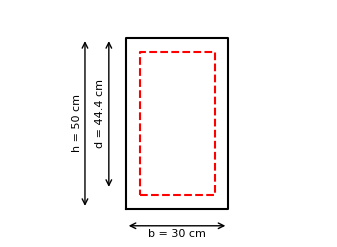
\includegraphics[height=5cm]{section.png}
\end{figure}

\end{minipage}

\vspace{0.5cm}


\section*{ Peralte: d (ART.1.1 E060) }

\[
d = h - d_e - \frac{1}{2} d_b - r
\]

\[
d = 50.0 - 0.95 - \frac{1}{2} 1.59 - 4.0
\]

\[
d = 44.25\,\text{cm}
\]

\vspace{0.5cm}

\section*{ Coeficiente B1 (ART.1.1 E060) }

\[
\beta_1 = 0.85
\]

\vspace{0.5cm}

\section*{ Pbal (ART.1.1 E060) }

\[
P_{bal}=\left(\frac{0.85 f_c \beta_1}{f_y}\right)\,\frac{6000}{6000+f_y}
\]

\[
P_{bal}=\left(\frac{0.85\,210.0\,0.850}{4200.0}\right)\,\frac{6000}{6000+4200.0}
\]

\[
P_{bal} = 0.0212
\]

\vspace{0.5cm}

\section*{ Pmax (ART.1.1 E060) }

\[
P_{max}=0.75\,P_{bal}
\]

\[
P_{max}=0.75\times0.0212
\]

\[
P_{max} = 0.0159
\]

\vspace{0.5cm}

\section*{ As mín (ART.1.1 E060) }

\[
A_s^{\text{min}} = 0.7\,\frac{\sqrt{f_c}}{f_y}\, b\, d
\]

\[
A_s^{\text{min}} = 0.7\,\frac{\sqrt{210.0}}{4200.0}\,30.0\,44.25
\]

\[
A_s^{\text{min}} = 3.21\,\text{cm}^2
\]

\vspace{0.5cm}

\section*{ As máx (ART.1.1 E060) }

\[
A_s^{\text{max}} = 0.75\,\left(\frac{0.85 f_c \beta_1}{f_y}\right)\,\left(\frac{6000}{6000+f_y}\right)\,b\,d
\]

\[
A_s^{\text{max}} = 21.16\,\text{cm}^2
\]

\vspace{0.5cm}

\section*{ Fórmula general del As (ART.1.1 E060) }

\[
A_s = \frac{1.7 f_c b d}{2 f_y} - \frac{1}{2} \sqrt{\frac{2.89(f_c b d)^2}{f_y^2} - \frac{6.8 f_c b M_u}{\phi f_y^2}}
\]

\vspace{0.5cm}

\section*{ As para M1- }

\[
M_u = -0.00\,\text{TN·m} = 0\,\text{kg·cm}
\]

\[
A_s^{\text{calc}} = -0.00\,\text{cm}^2
\]

\[
A_s^{\text{req}} = 3.21\,\text{cm}^2
\]

\vspace{0.5cm}

\section*{ As para M2- }

\[
M_u = -0.00\,\text{TN·m} = 0\,\text{kg·cm}
\]

\[
A_s^{\text{calc}} = -0.00\,\text{cm}^2
\]

\[
A_s^{\text{req}} = 3.21\,\text{cm}^2
\]

\vspace{0.5cm}

\section*{ As para M3- }

\[
M_u = -0.00\,\text{TN·m} = 0\,\text{kg·cm}
\]

\[
A_s^{\text{calc}} = -0.00\,\text{cm}^2
\]

\[
A_s^{\text{req}} = 3.21\,\text{cm}^2
\]

\vspace{0.5cm}

\section*{ As para M1+ }

\[
M_u = 0.00\,\text{TN·m} = 0\,\text{kg·cm}
\]

\[
A_s^{\text{calc}} = -0.00\,\text{cm}^2
\]

\[
A_s^{\text{req}} = 3.21\,\text{cm}^2
\]

\vspace{0.5cm}

\section*{ As para M2+ }

\[
M_u = 0.00\,\text{TN·m} = 0\,\text{kg·cm}
\]

\[
A_s^{\text{calc}} = -0.00\,\text{cm}^2
\]

\[
A_s^{\text{req}} = 3.21\,\text{cm}^2
\]

\vspace{0.5cm}

\section*{ As para M3+ }

\[
M_u = 0.00\,\text{TN·m} = 0\,\text{kg·cm}
\]

\[
A_s^{\text{calc}} = -0.00\,\text{cm}^2
\]

\[
A_s^{\text{req}} = 3.21\,\text{cm}^2
\]

\vspace{0.5cm}



\section*{Resultados}
\begin{tabular}{|l|c|}
\hline

As_min & 3.21 cm² \\

As_max & 21.16 cm² \\

As req M1- & 3.21 cm² \\

As req M2- & 3.21 cm² \\

As req M3- & 3.21 cm² \\

As req M1+ & 3.21 cm² \\

As req M2+ & 3.21 cm² \\

As req M3+ & 3.21 cm² \\

\hline
\end{tabular}



\begin{figure}[H]
\centering
\includegraphics[width=0.9\textwidth]{C:/Users/abemc/AppData/Local/Temp/view3d_tr_jmoux.png}
\end{figure}


\end{document}